\documentclass[a4paper,12pt]{book}
\usepackage{amsmath}
\usepackage[utf8]{inputenc}
\usepackage{pgfplots}
\usetikzlibrary{calc}

\title{Mathematics of Algorithms in libml}
\author{John Holly}
\date{\today}

\DeclareMathOperator{\arctanh}{arctanh}
\begin{document}

\maketitle

\tableofcontents

\chapter{Neurons}

\section{Stateful Components}

	\subsection{Weights}
	\text Weights are the unique part of a neuron that sway sets of inputs to one decision or the other. Training a neuron adjusts its weights to converge towards the training data it was provided.

	\subsection{Bias}
	\text There is often an extra weight in a neuron that plays an important role of moving the decision boundary (see Figure 1.1). The bias helps move the learned weights away from the origin so many inputs do not end up being represented by many of the same weights.

	\begin{figure}
	\begin{center}
	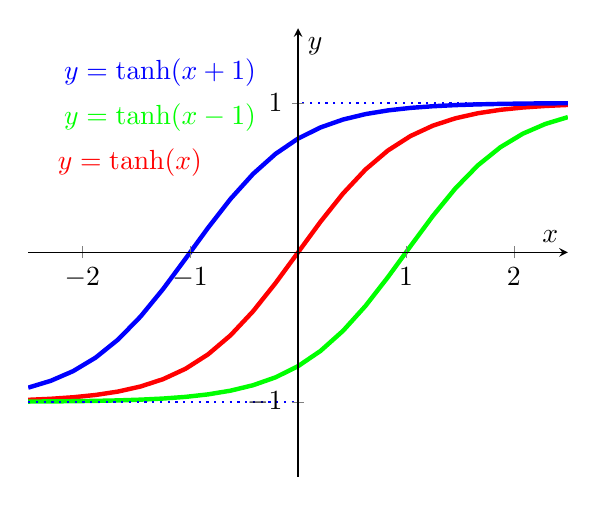
\begin{tikzpicture}
	\begin{axis}[
		xmin=-2.5, xmax=2.5,
		ymin=-1.5, ymax=1.5,
		axis lines=center,
		axis on top=true,
		domain=-2.5:2.5,
		ylabel=$y$,
		xlabel=$x$,
		]

		\addplot [mark=none,draw=red,ultra thick] {tanh(\x)};
		\addplot [mark=none,draw=green,ultra thick] {tanh(\x-1)};
		\addplot [mark=none,draw=blue,ultra thick] {tanh(\x+1)};
		\node [left, red] at (axis cs: -.8,.6) {$y = \tanh (x)$};
		\node [left, green] at (axis cs: -.3,.9) {$y = \tanh (x-1)$};
		\node [left, blue] at (axis cs: -.3,1.2) {$y = \tanh (x+1)$};

		%% Add the asymptotes
		\draw [blue, dotted, thick] (axis cs:-2.5,-1)-- (axis cs:0,-1);
		\draw [blue, dotted, thick] (axis cs:+2.5,+1)-- (axis cs:0,+1);
	\end{axis}
	\end{tikzpicture}
	\caption{Effect of bias on decision boundary}
	\end{center}
	\end{figure}

\section{Activation}
\text Neuron activation is the process of firing the neuron given some inputs. The neuron has fired if the activation is greater than or equal to 0.5.
\begin{align*}
	y = \arctanh(\sum_{i=1}^{n}{x}_i{w}_i+{b}), \\
	\text{where}~x &= \text{input,} \\
	w &= \text{corresponding weight,} \\
	b &= \text{bias weight}
\end{align*}

\section{Weight Adjustment}
\text Neurons are trained iteratively by feeding training data through and adjusting weights based on the error in regards to expected outcome.

	\subsection{Error calculation}
	\text As previously stated, the error is the difference between the expected and actual output of the neuron.
	\begin{align*}
		{e} = t-y, \\
		\text{where}~t &= \text{expected value} \\
	\end{align*}

	\subsection{Adjusting Weights}
	\text When an incorrect classification is made, the weights get adjusted in a direction to move future outputs closer to convergence. We introduce a learning rate to train faster and make greater steps in that direction. One needs to be careful not to make the steps too large and skip correct classifications.
	\begin{align*}
		{w}_i = {w}_i\cdot\eta\cdot{e}\cdot{x}_i, \\
		\text{where}~\eta &= \text{learning rate}
	\end{align*}

	\subsection{Adjusting Bias Weight}
	\text The bias weight is adjusted like regular weights but has no ties to a specific input.
	\begin{align*}
		b = b\cdot\eta\cdot{e}
	\end{align*}

\end{document}